%%%%%%%%%%%%%%%%%%%%%%%%%%%%%%%%%%%%%%%%%
% Medium Length Professional CV
% LaTeX Template
% Version 2.0 (8/5/13)
%
% This template has been downloaded from:
% http://www.LaTeXTemplates.com
%
% Original author:
% Rishi Shah 
%
% Important note:
% This template requires the resume.cls file to be in the same directory as the
% .tex file. The resume.cls file provides the resume style used for structuring the
% document.
%
%%%%%%%%%%%%%%%%%%%%%%%%%%%%%%%%%%%%%%%%%

%----------------------------------------------------------------------------------------
%	PACKAGES AND OTHER DOCUMENT CONFIGURATIONS
%----------------------------------------------------------------------------------------

\documentclass{resume} % Use the custom resume.cls style

%\usepackage{CJKutf8}

% \usepackage{mathspec}
% \setmathsfont{Times New Roman}
% \setmainfont{Times New Roman}
\usepackage[UTF8]{ctex}

\usepackage{url}
\usepackage{graphicx}


\usepackage[left=0.6in,top=0.5in,right=0.6in,bottom=0.5in]{geometry} % Document margins
\newcommand{\tab}[1]{\hspace{.2667\textwidth}\rlap{#1}}
\newcommand{\itab}[1]{\hspace{0em}\rlap{#1}}
\name{付振新}
\address{15650708568 \\ fuzhenxin95@gmail.com \\ \url{https://zhenxinfu.com}}
\address{GitHub: \url{https://github.com/fuzhenxin}}
% \address{注:目前已入职北京大学计算中心,不再找工作。}


\usepackage{tikz}
\usepackage{graphicx}
\usetikzlibrary{calc}



\begin{document}



\begin{tikzpicture}[remember picture,overlay]
    \node[anchor=south west,inner sep=0pt] at ($(current page.north east)-(4cm,4.2cm)$) {
       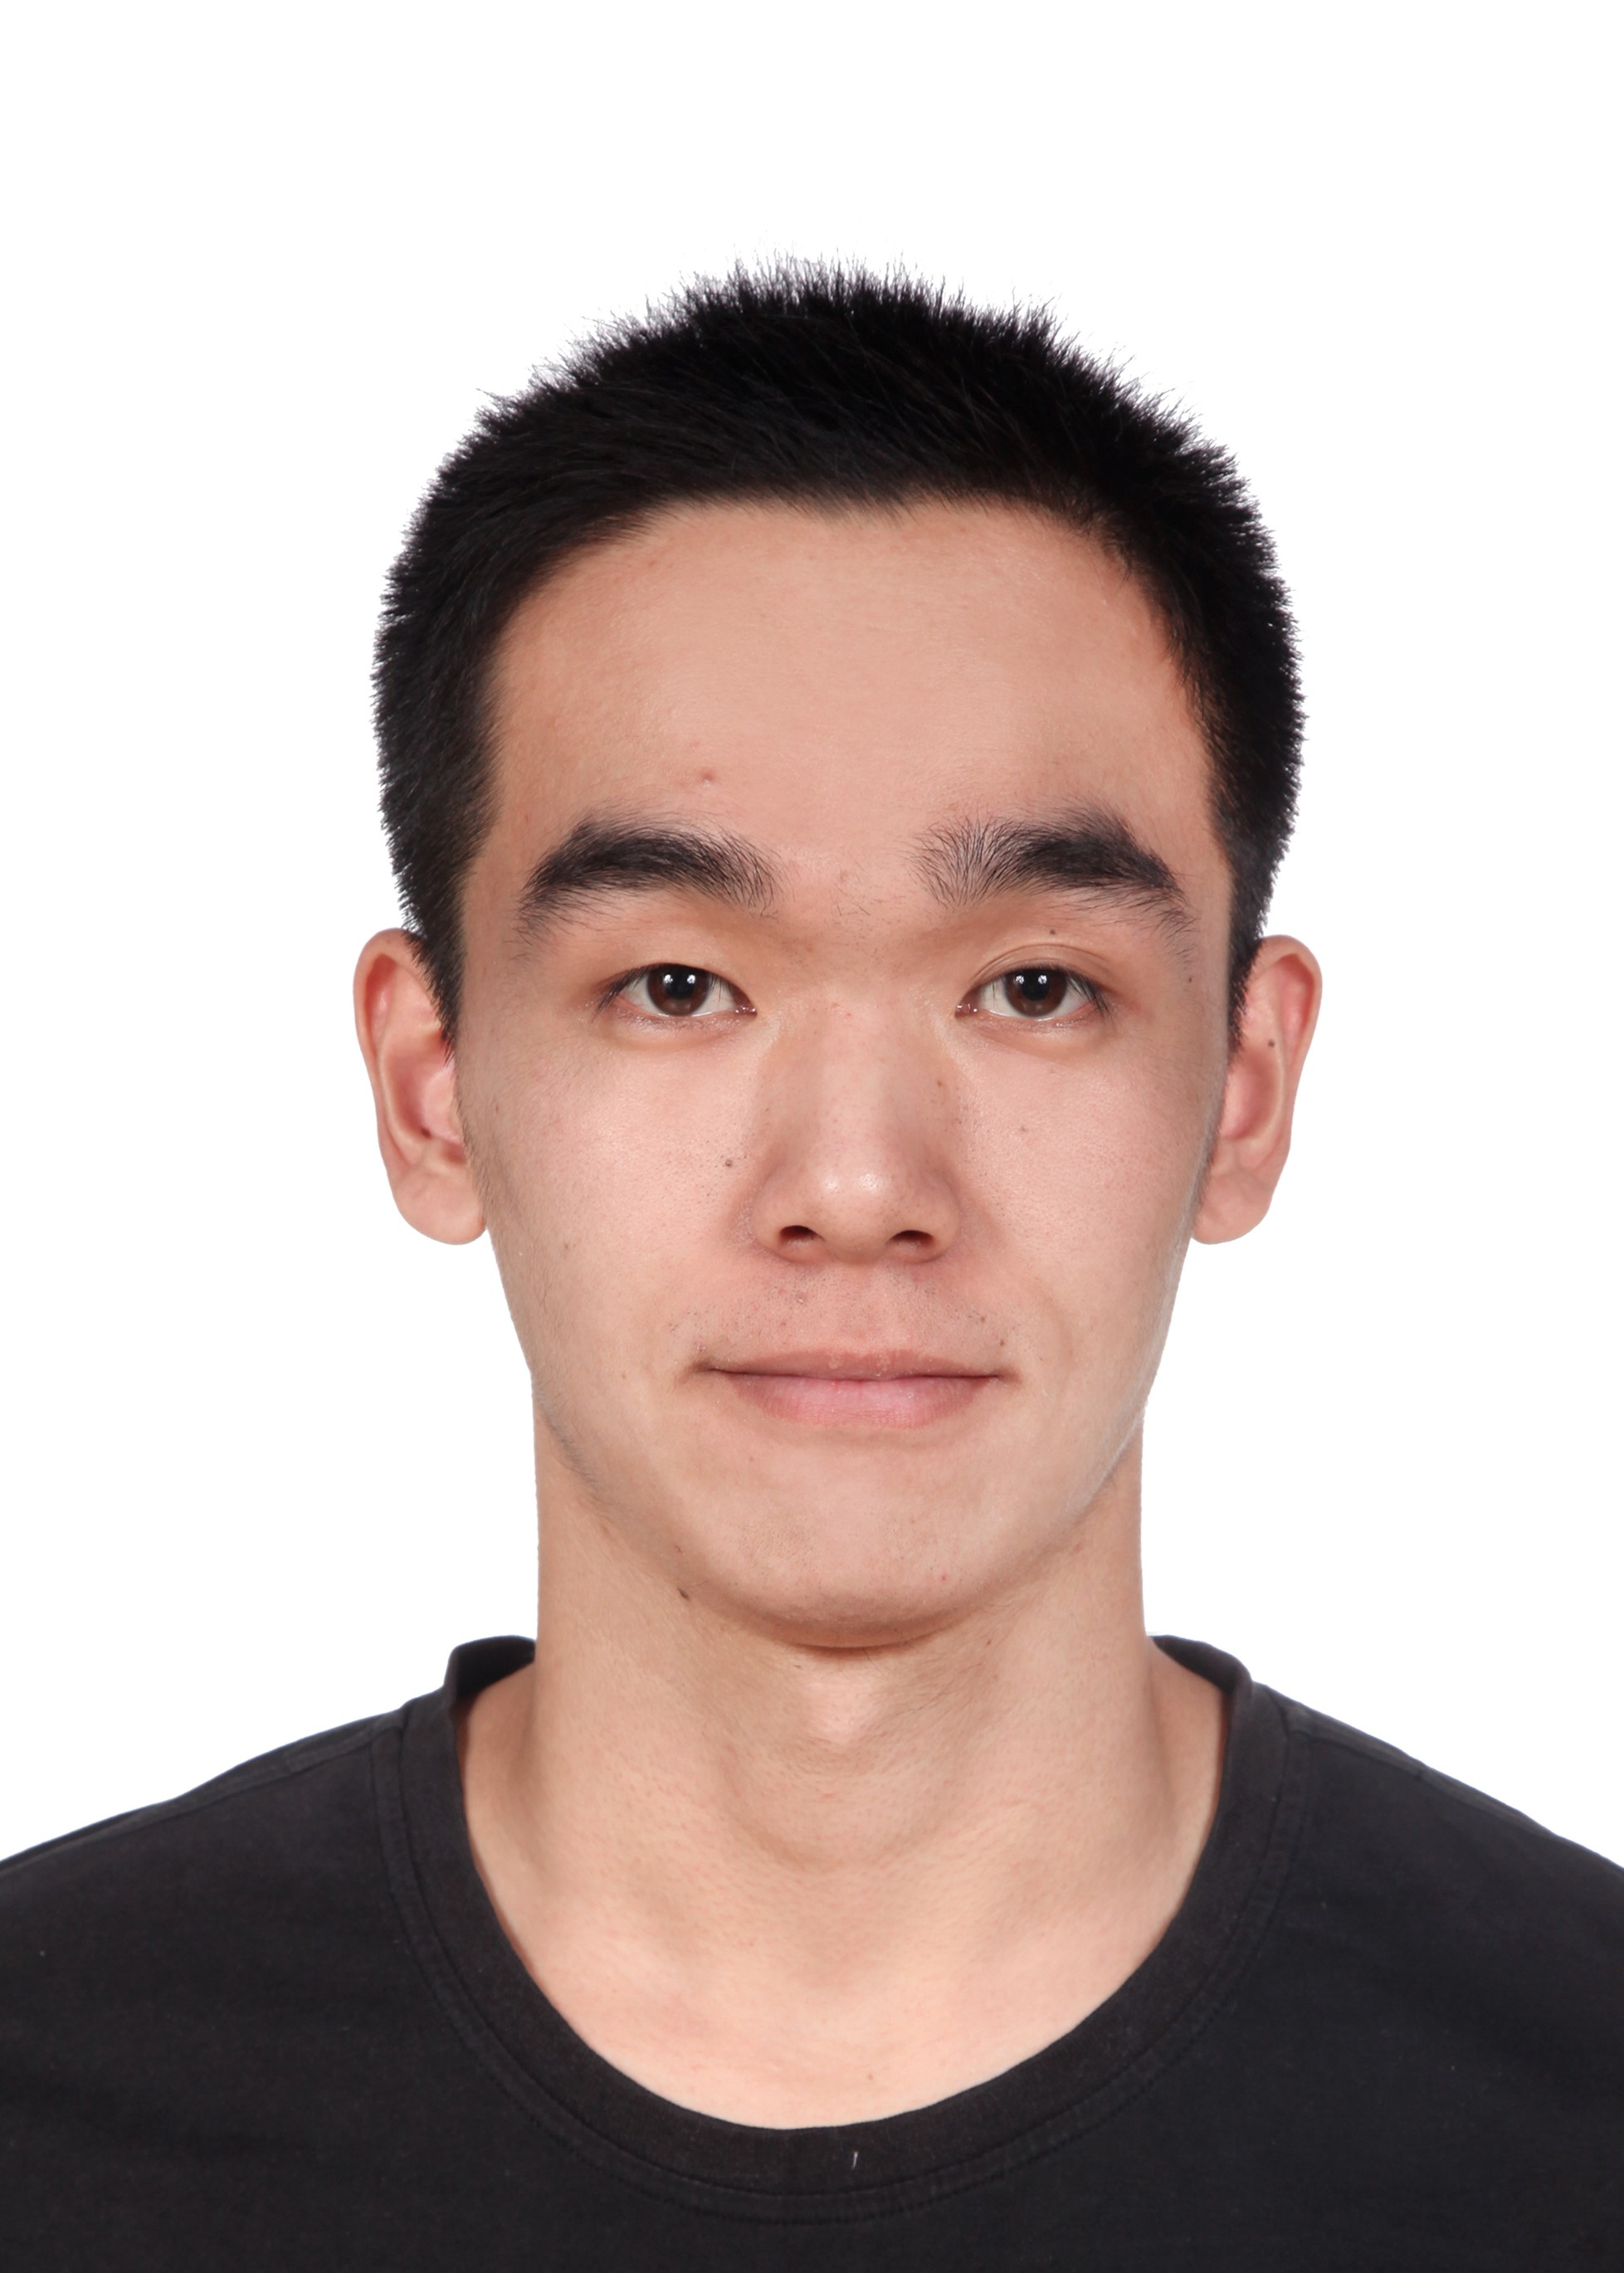
\includegraphics[width=0.12\columnwidth]{fzx.jpg}
    };
\end{tikzpicture}
\vspace{-9mm}


% \begin{rSection}{Education}

% {\bf Wangxuan Institute of Computer Technology (WICT), Peking University} \hfill {\em Sept 2018 - Present} 
% \\ Master in Natural Language Processing
% \\Formerly the institute of computer science and technology.\\
% {\bf School of Electronics Engineering and Computer Science, Peking University} \hfill {\em Sept 2014 - Jul 2018}
% \\ Bachelor of Computer Science
% \\ Department of Computer Science and Technology
% \end{rSection}

% \begin{rSection}{Competition and Internship}
% \textbf{Student Cluster Competition at SC16, SC17, ASC19, \& SC19} \hfill {\em Sept 2016 - Present}\\
% I am in charge of reproducing results of a given paper on our own cluster. We are selected to contribute to a special issue of the journal, Parallel Computing. In ASC19 and SC19, I worked as a coach. \\
% \textbf{Intern at Tencent Group} \hfill {\em Apr 2017 - Aug 2017} \\
% Test Engineer for virtual assistants and name entity recognition task using sequence labeling.\\
% \textbf{Intern at Alibaba Group} \hfill {\em Aug 2018 - Present}\\
% Research Intern for Natural Languge Processing in AliMe Team \& DAMO Academy.
% \end{rSection}

% \begin{rSection}{Publications}

%     [1] \textbf{Style Transfer in Text: Exploration and Evaluation}, AAAI, 2018. \textbf{Citation>100}\\
%     {\it \textbf{Zhenxin Fu}, Xiaoye Tan, Nanyun Peng, Dongyan Zhao, Rui Yan.} \\
%     We propose unsupervised sequence to sequence model to transfer text from style A to style B. For example, converting paper title to news title.

%     [2] \textbf{Query-bag Matching with Mutual Coverage for Information-seeking Conversations in E-commerce}, CIKM (Short), 2019. \\
%     {\it \textbf{Zhenxin Fu}, Feng Ji, Wenpeng Hu, Wei Zhou, Dongyan Zhao, Haiqing Chen, Rui Yan.} \\
%     A bag containing lots of questions corresponds to a same answer. Ranking the bag directly helps the information-seeking conversation.

%     [3] \textbf{Student Cluster Competition 2017, Team Peking University: Reproducing Vectorization of the Tersoff Multi-Body Potential on the Intel Broadwell Architecture}, Parallel Computing (Journel), 2018. \\
%     {\it \textbf{Zhenxin Fu}, Lei Yang, Wenbin Hou, Zhuohan Li, Yifan Wu, Yihua Cheng, Xiaolin Wang, Yun Liang.} \\
%     Report of reproducibility challenge for the student cluster competition at SC17.

%     [4] \textbf{Joint Learning of Word Representation and Sense Representation for Unsupervised Word Sense Disambiguation}, AAAI Student Abstract and Poster Program, 2020. \\
%     {\it Jie Wang, \textbf{Zhenxin Fu}, Moxin Li, Haisong Zhang, Dongyan Zhao, Rui Yan.} \\
%     Unsupervised WSD by learning the sense representation through the supervision from word embedding.

%     [5] \textbf{Semi-supervised Text Style Transfer: Cross Projection in Latent Space}, EMNLP-IJCNLP, 2019. \\
%     {\it Mingyue Shang, Piji Li, \textbf{Zhenxin Fu}, Lidong Bing, Dongyan Zhao, Shuming Shi, Rui Yan.} \\
%     Semi-supervsed text style transfer with cross projection in latent space: cross training autoencoder, style transfer and latent space projection.
    
%     [6] \textbf{Multilingual Dialogue Generation with Shared-Private Memory}, NLPCC (English), 2019. \textbf{Outstanding Paper Award}. \\
%     {\it Chen Chen, Lisong Qiu, \textbf{Zhenxin Fu}, Junfei Li, Rui Yan. } \\
%     Multilingual dailog generation with shared-private memory inspired from multi-task learning.
    
%     [7] \textbf{Automated ICD Coding Based on Word Embedding with Entry Embedding and Attention Mechanism (基于融合条目词嵌入和注意力机制的自动ICD编码)}, NLPCC (Chinese), 2019. \\
%     {\it Hongke Zhang, \textbf{Zhenxin Fu}, Qianping Ren, Hui Xu, Dongyan Zhao, Rui Yan.} \\
%     A classification model for International Classification of Disease (ICD) with item embedding and label attention.

%     [8] \textbf{Find a Reasonable Ending for Stories: Does Logic Relation Help the Story Cloze Test?} AAAI Student Abstract and Poster Program, 2019. \\
%     {\it Mingyue Shang, \textbf{Zhenxin Fu}, Hongzhi Yin, Bo Tang, Dongyan Zhao, Rui Yan.} \\
%     Natural language inference is used to promote story cloze test.
    
%     [9] \textbf{Learning to Converse with Noisy Data: Generation with Calibration}, IJCAI-ECAI, 2018. \\
%     {\it Mingyue Shang, \textbf{Zhenxin Fu}, Nanyun Peng, Yansong Feng, Dongyan Zhao, Rui Yan.}  \\
%     Noise training cases harm trainnig process of generation-based dialog system. So we integrate instance weight into dialog system to overcome the problem.

%     [10] \textbf{One "Ruler" for All Languages: Multi-Lingual Dialogue Evaluation with Adversarial Multi-Task Learning}, IJCAI-ECAI, 2018. \\
%     {\it Xiaowei Tong, \textbf{Zhenxin Fu}, Mingyue Shang, Dongyan Zhao, Rui Yan.} \\
%     We apply multi-task learning in open-domain dialog evaluation.

%     [11] \textbf{ParConnect Reproducibility Report}, Parallel Computing (Journal), 2017.\\
%     {\it Lei Yang, Yilong Li, \textbf{Zhenxin Fu}, Zhuohan Li, Wenbin Hou, Haoze Wu, Xiaolin Wang, Yun Liang.} \\
%     The report of reproducibility challenge for the student cluster competition at SC16.


% \end{rSection}


% \begin{rSection}{Others}
% \textbf{Reviewer}: AAAI-2019; ACL-2019; EMNLP-2019; INLG-2019; AAAI-2020, ACL-2020. \\
% \textbf{Teaching assistant}: Introduction to Natural Language Processing: Foundation, Theory and Application, Spring 2019. \\
% \textbf{Scholarship}: [1] Wang Xuan Scholarship, first prize for the undergraduate internship at ICST, 2018; [2] Special Scholarship (7/32), Peking University, 2019. \\
% \textbf{Github}: A paper list for style transfer in text with star>700. Link: \url{https://github.com/fuzhenxin/Style-Transfer-in-Text}\\
% \textbf{Simple Chrome Extension}: A very simple "Chrome Extension" to automatically log in official websites in PKU (iaaa.pku.edu.cn).

% \end{rSection}

% \begin{rSection}{简介}
%     付振新,天津人,本科和硕士均就读于北京大学,\\
%     \textbf{研究方向}: 自然语言处理, 主要研究方向为文本生成和文本匹配,包括生成式对话系统、文本风格迁移,和检索式对话系统,研究成果发表在KDD,AAAI,SIGIR,IJCAI,EMNLP,CIKM,NLPCC等相关会议上。

% \end{rSection}

\begin{rSection}{教育和工作经历}
    {\bf 北京大学计算中心} \hfill {\em 2021年7月 - 今~~~~~~~~~~~~~} 
    \\ 助理工程师:高性能计算、自然语言处理 \\
    {\bf 北京大学王选计算机研究所(原北京大学计算机科学技术研究所)} \hfill {\em 2018年9月 - 2021年7月} 
    \\ 硕士:计算机应用技术,自然语言处理 \\
    {\bf 北京大学信息科学技术学院} \hfill {\em 2014年9月 - 2018年7月}
    \\ 学士:计算机科学与技术,自然语言处理
\end{rSection}

\vspace{-0.2cm}
\begin{rSection}{竞赛和实习经历}
    \textbf{大学生超算竞赛(SC16, SC17, ASC19, SC19, SC20, ASC20-21 \& SC21)} \hfill {\em 2016年9月 - 2021年7月}\\
    本科期间负责复现高性能计算论文子任务,在SC16、SC17世界大学生超算比赛分别获团体第六、第四名。
    研究生与工作期间作为教练组织日常训练,带队参加了多次国际比赛,并在SC20获得第二名。 \\
    \textbf{腾讯} \hfill {\em 2017年4月 - 2017年8月} \\
    智能助手的测试\&负责一个车载语音导航项目的地名识别工作(命名实体识别)。\\
    \textbf{阿里巴巴} \hfill {\em 2018年8月 - 2020年6月}\\
    达摩院阿里小蜜团队研究型实习生,实习期间主要做检索式对话系统的研究工作,共发表三篇论文。
\end{rSection}

\vspace{-0.2cm}
\begin{rSection}{研究方向:自然语言处理}
    \textbf{文本生成:}文本风格迁移(AAAI2018,EMNLP2019),生成式对话系统(IJCAI2018,IJCAI2018,NLPCC2019) \\
    \textbf{文本匹配:}检索式对话系统(CIKM2019,KDD2020,CIKM2020),故事结尾预测(AAAI2019),词义消歧(AAAI2020)
\end{rSection}

\vspace{-0.2cm}
\begin{rSection}{论文(三篇CCF-A类一作(含一篇共同一作),三篇CCF-B类一作(含一篇短文))}
    % \textbf{研究方向:自然语言处理}
    % \begin{itemize}
    %     \item 文本生成:文本风格迁移,生成式对话系统
    %     \item 文本匹配:检索式对话系统
    % \end{itemize}

    [1] \textbf{Style Transfer in Text: Exploration and Evaluation}, AAAI, 2018. \textbf{引用数259}.\\
    {\it \textbf{Zhenxin Fu}, Xiaoye Tan, Nanyun Peng, Dongyan Zhao, Rui Yan.} \\
    较早的提出无监督场景下的文本风格迁移模型并提出评价指标。
    \vspace{-0.1cm}
  
    [2] \textbf{Context-to-Session Matching: Utilizing Whole Session for Response Selection in Information-Seeking Dialogue Systems}, KDD, 2020. \\
    {\it \textbf{Zhenxin Fu}, Shaobo Cui, Mingyue Shang, Feng Ji, Dongyan Zhao, Haiqing Chen, Rui Yan.} \\
    讲问题-问题匹配和问题-答案匹配这两个客服类对话中的关键点结合在一起,模型上提出多句-多句匹配模型。
    \vspace{-0.1cm}

    [3] \textbf{Query-to-Session Matching: Do NOT Forget History and Future during Response Selection for Multi-Turn Dialogue Systems}, CIKM, 2020. \\
    {\it \textbf{Zhenxin Fu}, Shaobo Cui, Feng Ji, Ji Zhang, Haiqing Chen, Dongyan Zhao, Rui Yan.}\\
    综合考虑了检索式对话中,候选回复以及它的前文和后文,模型上建模了对话中的对话流关系。
    \vspace{-0.1cm}
    
    [4] \textbf{Query-bag Matching with Mutual Coverage for Information-seeking Conversations in E-commerce}, CIKM (Short), 2019. \\
    {\it \textbf{Zhenxin Fu}, Feng Ji, Wenpeng Hu, Wei Zhou, Dongyan Zhao, Haiqing Chen, Rui Yan.}\\
    在问题-问题匹配的场景下,将候选问题扩展为包括该问题不同表述的问题包,模型上提出互相覆盖模型。
    \vspace{-0.1cm}

    [5] \textbf{Be Aware of the Hot Zone: A Warning System of Hazard Area Prediction to Intervene Novel Coronavirus COVID-19 Outbreak}, SIGIR Industry Track, 10 pages, 2020. \\
    {\it \textbf{Zhenxin Fu}$^*$, Yu Wu$^*$, Hailei Zhang, Yichuan Hu, Dongyan Zhao, Rui Yan..}\\
    利用新冠肺炎公布确诊病例地点时间数据,进行任意地点的危险程度预测。
    \vspace{-0.1cm}

    [6] \textbf{Student Cluster Competition 2017, Team Peking University: Reproducing Vectorization of the Tersoff Multi-Body Potential on the Intel Broadwell Architecture}, Parallel Computing, 2018. \\
    {\it \textbf{Zhenxin Fu}, Lei Yang, Wenbin Hou, Zhuohan Li, Yifan Wu, Yihua Cheng, Xiaolin Wang, Yun Liang.} \\
    SC2017大学生超算比赛的论文复现报告,受邀投稿该期刊。
    \vspace{-0.1cm}

    [7] \textbf{Learning to Converse with Noisy Data: Generation with Calibration}, IJCAI-ECAI, 2018. \\
    {\it Mingyue Shang, \textbf{Zhenxin Fu}, Nanyun Peng, Yansong Feng, Dongyan Zhao, Rui Yan.} 
    \vspace{-0.1cm}

    [8] \textbf{One ``Ruler" for All Languages: Multi-Lingual Dialogue Evaluation with Adversarial Multi-Task Learning}, IJCAI-ECAI, 2018. \\
    {\it Xiaowei Tong, \textbf{Zhenxin Fu}, Mingyue Shang, Dongyan Zhao, Rui Yan.}
    \vspace{-0.1cm}

    [9] \textbf{Find a Reasonable Ending for Stories: Does Logic Relation Help the Story Cloze Test?} AAAI Student Abstract and Poster Program, 2019. \\
    {\it Mingyue Shang, \textbf{Zhenxin Fu}, Hongzhi Yin, Bo Tang, Dongyan Zhao, Rui Yan.}
    \vspace{-0.1cm}

    [10] \textbf{Learning Sense Representation from Word Representation for Unsupervised Word Sense Disambiguation}, AAAI Student Abstract and Poster Program, 2020. \\
    {\it Jie Wang, \textbf{Zhenxin Fu}, Moxin Li, Haisong Zhang, Dongyan Zhao, Rui Yan.}
    \vspace{-0.1cm}

    [11] \textbf{Automated ICD Coding Based on Word Embedding with Entry Embedding and Attention Mechanism (基于融合条目词嵌入和注意力机制的自动ICD编码)}, NLPCC (Chinese), 2019. \\
    {\it Hongke Zhang, \textbf{Zhenxin Fu}, Qianping Ren, Hui Xu, Dongyan Zhao, Rui Yan.}
    \vspace{-0.1cm}

    [12] \textbf{Semi-supervised Text Style Transfer: Cross Projection in Latent Space}, EMNLP-IJCNLP, 2019. \\
    {\it Mingyue Shang, Piji Li, \textbf{Zhenxin Fu}, Lidong Bing, Dongyan Zhao, Shuming Shi, Rui Yan.}
    \vspace{-0.1cm}

    [13] \textbf{Multilingual Dialogue Generation with Shared-Private Memory}, NLPCC (English), 2019. \\
    {\it Chen Chen, Lisong Qiu, \textbf{Zhenxin Fu}, Junfei Li, Rui Yan. }
    \vspace{-0.1cm}

    [14] \textbf{ParConnect Reproducibility Report}, Parallel Computing, 2017.\\
    {\it Lei Yang, Yilong Li, \textbf{Zhenxin Fu}, Zhuohan Li, Wenbin Hou, Haoze Wu, Xiaolin Wang, Yun Liang.}
    \vspace{-0.1cm}

    [15] \textbf{Critique of ``Computing Planetary Interior Normal Modes with a Highly Parallel Polynomial Filtering Eigensolver" by SCC Team from Peking University}, IEEE TPDS Special Issue about Reproducibility, 2021. \\
    {\it Yihua Cheng, Zejia Fan, Jing Mai, Yifan Wu, Pengcheng Xu, Yuxuan Yan, \textbf{Zhenxin Fu}, Yun Liang.}
    \vspace{-0.1cm}
\end{rSection}

\vspace{-0.2cm}
\begin{rSection}{其他}
    \textbf{技能}: Python, C/C++, Java, 按技能熟练程度排序. \\
    \textbf{审稿人}: AAAI-2019/2020/2021; ACL-2019/2020/2021; EMNLP-2019/2020; INLG-2019; COLING-2020. \\
    \textbf{Senior Program Committee}: IJCAI 2021. \\
    \textbf{奖学金}: [1] 王选奖学金,一等奖, 2018. [2] 专项奖学金 (7/32), 北京大学, 2019. [3] 国家奖学金 (1/24), 2020.\\
    \textbf{奖励}: [1] 北京大学``赛帕斯''杯程序设计竞赛, 三等奖, 2016. [2] 优秀科研奖 (7/32),北京大学, 2019. [3] NLPCC Outstanding Paper Award,2019 [4] 三好学生标兵, 2020. [5]学术创新奖 (2/150), 北京大学.\\
    \textbf{GitHub}: 文本风格迁移论文列表。GitHub中Star数超过一千. \\链接: \url{https://github.com/fuzhenxin/Style-Transfer-in-Text}\\
    \textbf{Mirror Site}: 构建北京大学开源镜像站. 链接: \url{https://mirrors.pku.edu.cn}
\end{rSection}

\end{document}
